\chapter{Further MNIST Interpretations}
\label{section:moremnistinterp}

\begin{figure}[ht]
    \centering
    \begin{subfigure}[b]{0.47\textwidth}
        \centering
        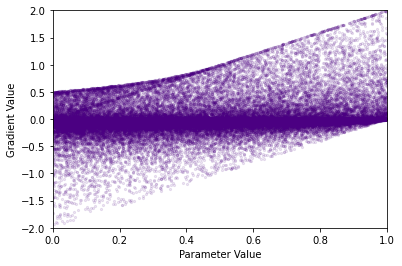
\includegraphics[width=\textwidth]{imgs/grad_prod_2_falseparam.png}
        \caption{Gradient samples for correct parameter $\F$}
        \label{fig:conjgrad2false}
    \end{subfigure}
    \begin{subfigure}[b]{0.47\textwidth}
        \centering
        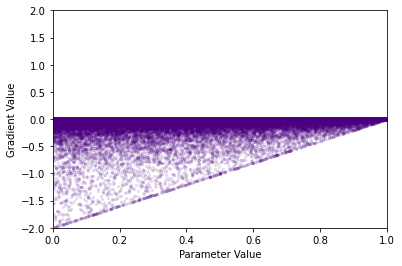
\includegraphics[width=\textwidth]{imgs/grad_prod_2_trueparam.png}
        \caption{Gradient samples for correct parameter $\T$}
        \label{fig:conjgrad2true}
    \end{subfigure}
    \begin{subfigure}[b]{0.47\textwidth}
        \centering
        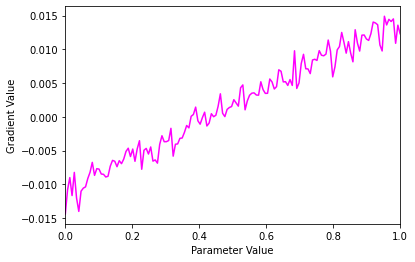
\includegraphics[width=\textwidth]{imgs/grad_prod_2_falseparam_avg.png}
        \caption{Mean gradient estimator for correct parameter $\F$}
        \label{fig:conjgrad2falseavg}
    \end{subfigure}
    \begin{subfigure}[b]{0.47\textwidth}
        \centering
        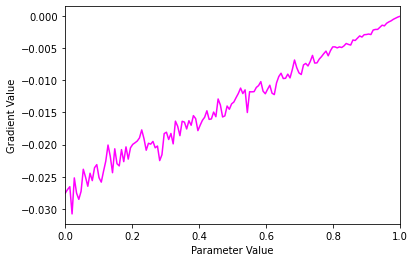
\includegraphics[width=\textwidth]{imgs/grad_prod_2_trueparam_avg.png}
        \caption{Mean gradient estimator for correct parameter $\T$}
        \label{fig:conjgrad2trueavg}
    \end{subfigure}
       \caption{Gradient estimations over the problem of real conjunctions with $\XOR$ loss $a=2$. We begin to see a separation between parameters, though the value of parameters with true value $\F$ seem to converge around 0.4, due to class imbalance.}
       \label{fig:conjgrad2}
\end{figure}